
%%%%%%%%%%%% MID WAY AGENDA %%%%%%%%%%%%%%
% \begin{frame}<beamer>
% \frametitle{Ignacio Trojaola Bolinaga}
% \tableofcontents[currentsection]
% \end{frame}
%%%%%%%%%%%% MID WAY AGENDA %%%%%%%%%%%%%%

\subsection{Parameter identification}

\begin{frame}{Modelling}{Parameter identification}
\begin{itemize}
	\item<1-> Nonlinear parameter identification
	\item<1-> Linearization of the model 
	\item<1-> Linear parameter identification
\end{itemize}
\end{frame}

\subsection{State-space model for control}

\begin{frame}{Modelling}{State-space model for control}
\begin{itemize}
	\item<1-> Discretization 
	\item<1-> Setting up on standard state-space fomrm
\end{itemize}
\end{frame}

\subsection{Verification of model}

\begin{frame}{Modelling}{Verification of model}
\begin{itemize}
	\item<1-> Compared model to real system
	\begin{itemize}
		\item<1-> Time constant 
		\item<1-> Behavior then applying a non-zero input
	\end{itemize}
\end{itemize}
\begin{itemize}
	\item<1-> The model behave as expected
\end{itemize}

\begin{figure}[H]
   \centering
    % This file was created by matlab2tikz.
%
%The latest updates can be retrieved from
%  http://www.mathworks.com/matlabcentral/fileexchange/22022-matlab2tikz-matlab2tikz
%where you can also make suggestions and rate matlab2tikz.
%
\definecolor{mycolor1}{rgb}{1.00000,1.00000,0.06667}%
\definecolor{mycolor2}{rgb}{0.07451,0.62353,1.00000}%
\definecolor{mycolor3}{rgb}{1.00000,0.41176,0.16078}%
\definecolor{mycolor4}{rgb}{0.68627,0.68627,0.68627}%
%
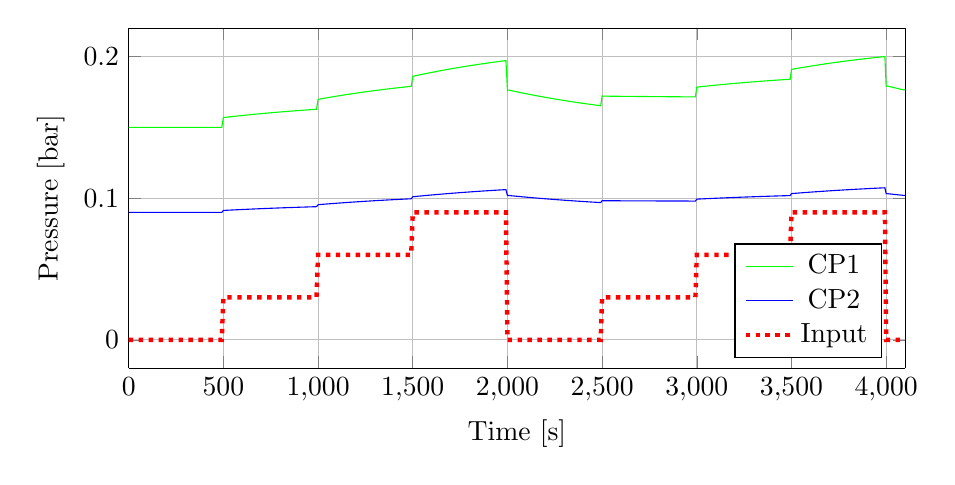
\begin{tikzpicture}

\begin{axis}[%
scaled y ticks = false,
 y tick label style={/pgf/number format/fixed,
/pgf/number format/1000 sep = \thinspace}, % Optional if you want to replace comma as the 1000 separator 
width=3.882in,
height=1.7in,
at={(0.303in,0.41in)},
scale only axis,
separate axis lines,
every outer x axis line/.append style={black},
every x tick label/.append style={font=\color{black}},
xmin=0,
xmax=4100,
xlabel={Time [s]},
xmajorgrids,
every outer y axis line/.append style={black},
every y tick label/.append style={font=\color{black}},
ymin=-0.02,
ymax=0.22,
ymajorgrids,
ylabel={Pressure [bar]},
legend pos=south east,
axis background/.style={fill=white}
]
\addplot [color=green,solid]
  table[row sep=crcr]{
0	0.15\\
8.93323388268949	0.15\\
17.866467765379	0.15\\
26.7997016480685	0.15\\
35.732935530758	0.15\\
44.6661694134474	0.15\\
53.5994032961369	0.15\\
62.5326371788264	0.15\\
71.4658710615159	0.15\\
80.3991049442054	0.15\\
89.3323388268949	0.15\\
98.2655727095844	0.15\\
107.198806592274	0.15\\
116.132040474963	0.15\\
125.065274357653	0.15\\
133.998508240342	0.15\\
142.931742123032	0.15\\
151.864976005721	0.15\\
160.798209888411	0.15\\
169.7314437711	0.15\\
178.66467765379	0.15\\
187.597911536479	0.15\\
196.531145419169	0.15\\
205.464379301858	0.15\\
214.397613184548	0.15\\
223.330847067237	0.15\\
232.264080949927	0.15\\
241.197314832616	0.15\\
250.130548715306	0.15\\
259.063782597995	0.15\\
267.997016480685	0.15\\
276.930250363374	0.15\\
285.863484246064	0.15\\
294.796718128753	0.15\\
303.729952011443	0.15\\
312.663185894132	0.15\\
321.596419776822	0.15\\
330.529653659511	0.15\\
339.462887542201	0.15\\
348.39612142489	0.15\\
357.32935530758	0.15\\
366.262589190269	0.15\\
375.195823072959	0.15\\
384.129056955648	0.15\\
393.062290838338	0.15\\
401.995524721027	0.15\\
410.928758603717	0.15\\
419.861992486406	0.15\\
428.795226369095	0.15\\
437.728460251785	0.15\\
446.661694134474	0.15\\
455.594928017164	0.15\\
464.528161899853	0.15\\
473.461395782543	0.15\\
482.394629665232	0.15\\
491.327863547922	0.15\\
500	0.156936442437769\\
500.261097430611	0.156936442437769\\
509.194331313301	0.15707406453234\\
518.12756519599	0.157210317263982\\
527.06079907868	0.157345214258088\\
535.994032961369	0.157478769004471\\
544.927266844059	0.157610994858723\\
553.860500726748	0.157741905043543\\
562.793734609438	0.157871512650062\\
571.726968492127	0.157999830639154\\
580.660202374817	0.158126871842727\\
589.593436257506	0.158252648965012\\
598.526670140196	0.158377174583831\\
607.459904022885	0.158500461151851\\
616.393137905575	0.158622520997838\\
625.326371788264	0.15874336632788\\
634.259605670954	0.158863009226615\\
643.192839553643	0.158981461658436\\
652.126073436333	0.159098735468689\\
661.059307319022	0.159214842384857\\
669.992541201712	0.15932979401773\\
678.925775084401	0.159443601862572\\
687.859008967091	0.159556277300265\\
696.79224284978	0.159667831598451\\
705.72547673247	0.159778275912656\\
714.658710615159	0.159887621287406\\
723.591944497849	0.159995878657334\\
732.525178380538	0.160103058848269\\
741.458412263228	0.160209172578324\\
750.391646145917	0.160314230458964\\
759.324880028607	0.160418242996066\\
768.258113911296	0.160521220590976\\
777.191347793986	0.16062317354154\\
786.124581676675	0.160724112043143\\
795.057815559364	0.160824046189721\\
803.991049442054	0.160922985974776\\
812.924283324744	0.161020941292372\\
821.857517207433	0.161117921938124\\
830.790751090123	0.161213937610182\\
839.723984972812	0.161308997910195\\
848.657218855501	0.161403112344276\\
857.590452738191	0.161496290323949\\
866.52368662088	0.161588541167093\\
875.45692050357	0.161679874098871\\
884.390154386259	0.161770298252656\\
893.323388268949	0.161859822670942\\
902.256622151638	0.161948456306247\\
911.189856034328	0.162036208022011\\
920.123089917017	0.162123086593483\\
929.056323799707	0.162209100708593\\
937.989557682396	0.162294258968829\\
946.922791565086	0.162378569890088\\
955.856025447775	0.162462041903538\\
964.789259330465	0.16254468335645\\
973.722493213154	0.162626502513042\\
982.655727095844	0.1627075075553\\
991.588960978533	0.162787706583798\\
1000	0.169724149021567\\
1000.52219486122	0.169803550056277\\
1009.45542874391	0.170019783131943\\
1018.3886626266	0.17023386465223\\
1027.32189650929	0.170445816025477\\
1036.25513039198	0.170655658447002\\
1045.18836427467	0.170863412901231\\
1054.12159815736	0.171069100163787\\
1063.05483204005	0.171272740803574\\
1071.98806592274	0.171474355184833\\
1080.92129980543	0.171673963469175\\
1089.85453368812	0.171871585617602\\
1098.78776757081	0.172067241392499\\
1107.7210014535	0.172260950359612\\
1116.65423533619	0.172452731890007\\
1125.58746921888	0.172642605162\\
1134.52070310157	0.172830589163084\\
1143.45393698425	0.173016702691821\\
1152.38717086694	0.173200964359725\\
1161.32040474963	0.173383392593121\\
1170.25363863232	0.173564005634991\\
1179.18687251501	0.173742821546794\\
1188.1201063977	0.173919858210277\\
1197.05334028039	0.174095133329259\\
1205.98657416308	0.174268664431403\\
1214.91980804577	0.174440468869969\\
1223.85304192846	0.174610563825549\\
1232.78627581115	0.174778966307786\\
1241.71950969384	0.174945693157073\\
1250.65274357653	0.17511076104624\\
1259.58597745922	0.175274186482218\\
1268.51921134191	0.175435985807692\\
1277.4524452246	0.175596175202734\\
1286.38567910729	0.175754770686422\\
1295.31891298998	0.175911788118441\\
1304.25214687267	0.17606724320067\\
1313.18538075535	0.176221151478752\\
1322.11861463804	0.176373528343648\\
1331.05184852073	0.176524389033175\\
1339.98508240342	0.176673748633532\\
1348.91831628611	0.17682162208081\\
1357.8515501688	0.17696802416248\\
1366.78478405149	0.177112969518877\\
1375.71801793418	0.177256472644662\\
1384.65125181687	0.177398547890271\\
1393.58448569956	0.177539209463352\\
1402.51771958225	0.177678471430183\\
1411.45095346494	0.177816347717082\\
1420.38418734763	0.177952852111796\\
1429.31742123032	0.178087998264883\\
1438.25065511301	0.178221799691074\\
1447.1838889957	0.178354269770628\\
1456.11712287839	0.178485421750667\\
1465.05035676108	0.178615268746503\\
1473.98359064377	0.178743823742948\\
1482.91682452646	0.178871099595611\\
1491.85005840914	0.178997109032188\\
1500	0.185933551469957\\
1500.78329229183	0.186058307091501\\
1509.71652617452	0.186319443468253\\
1518.64976005721	0.186577981494248\\
1527.5829939399	0.186833947023512\\
1536.51622782259	0.187087365652819\\
1545.44946170528	0.187338262724251\\
1554.38269558797	0.187586663327732\\
1563.31592947066	0.187832592303537\\
1572.24916335335	0.188076074244775\\
1581.18239723604	0.188317133499851\\
1590.11563111873	0.1885557941749\\
1599.04886500142	0.188792080136193\\
1607.98209888411	0.189026015012533\\
1616.9153327668	0.189257622197608\\
1625.84856664949	0.189486924852337\\
1634.78180053218	0.189713945907184\\
1643.71503441487	0.18993870806445\\
1652.64826829756	0.190161233800545\\
1661.58150218025	0.190381545368235\\
1670.51473606293	0.190599664798868\\
1679.44796994562	0.190815613904573\\
1688.38120382831	0.191029414280449\\
1697.314437711	0.191241087306719\\
1706.24767159369	0.191450654150866\\
1715.18090547638	0.191658135769757\\
1724.11413935907	0.191863552911734\\
1733.04737324176	0.192066926118686\\
1741.98060712445	0.192268275728112\\
1750.91384100714	0.192467621875146\\
1759.84707488983	0.192664984494574\\
1768.78030877252	0.192860383322829\\
1777.71354265521	0.193053837899963\\
1786.6467765379	0.193245367571601\\
1795.58001042059	0.193434991490875\\
1804.51324430328	0.193622728620341\\
1813.44647818597	0.193808597733874\\
1822.37971206866	0.193992617418545\\
1831.31294595135	0.194174806076484\\
1840.24617983403	0.194355181926711\\
1849.17941371672	0.194533763006969\\
1858.11264759941	0.19471056717552\\
1867.0458814821	0.194885612112933\\
1875.97911536479	0.195058915323853\\
1884.91234924748	0.195230494138752\\
1893.84558313017	0.195400365715658\\
1902.77881701286	0.195568547041876\\
1911.71205089555	0.195735054935684\\
1920.64528477824	0.195899906048015\\
1929.57851866093	0.196063116864124\\
1938.51175254362	0.196224703705231\\
1947.44498642631	0.196384682730162\\
1956.378220309	0.196543069936957\\
1965.31145419169	0.196699881164473\\
1974.24468807438	0.196855132093969\\
1983.17792195707	0.197008838250671\\
1992.11115583976	0.197161015005328\\
2000	0.176351687692023\\
2001.04438972245	0.176502350262442\\
2009.97762360514	0.176238647431297\\
2018.91085748782	0.175977568487561\\
2027.84409137051	0.175719087323113\\
2036.7773252532	0.175463178089615\\
2045.71055913589	0.175209815195921\\
2054.64379301858	0.174958973305523\\
2063.57702690127	0.174710627334017\\
2072.51026078396	0.174464752446589\\
2081.44349466665	0.174221324055539\\
2090.37672854934	0.173980317817817\\
2099.30996243203	0.173741709632593\\
2108.24319631472	0.17350547563884\\
2117.17643019741	0.173271592212955\\
2126.1096640801	0.173040035966394\\
2135.04289796279	0.172810783743333\\
2143.97613184548	0.17258381261835\\
2152.90936572817	0.172359099894138\\
2161.84259961086	0.172136623099229\\
2170.77583349355	0.171916359985752\\
2179.70906737624	0.171698288527206\\
2188.64230125892	0.171482386916256\\
2197.57553514161	0.171268633562554\\
2206.5087690243	0.171057007090581\\
2215.44200290699	0.170847486337507\\
2224.37523678968	0.170640050351075\\
2233.30847067237	0.170434678387507\\
2242.24170455506	0.17023134990943\\
2251.17493843775	0.170030044583821\\
2260.10817232044	0.169830742279972\\
2269.04140620313	0.169633423067481\\
2277.97464008582	0.169438067214257\\
2286.90787396851	0.169244655184546\\
2295.8411078512	0.169053167636976\\
2304.77434173389	0.16886358542263\\
2313.70757561658	0.16867588958312\\
2322.64080949927	0.168490061348701\\
2331.57404338196	0.168306082136389\\
2340.50727726465	0.168123933548104\\
2349.44051114734	0.16794359736883\\
2358.37374503003	0.167765055564792\\
2367.30697891271	0.167588290281657\\
2376.2402127954	0.167413283842744\\
2385.17344667809	0.167240018747256\\
2394.10668056078	0.167068477668536\\
2403.03991444347	0.166898643452326\\
2411.97314832616	0.16673049911506\\
2420.90638220885	0.166564027842157\\
2429.83961609154	0.166399212986346\\
2438.77284997423	0.166236038066\\
2447.70608385692	0.166074486763486\\
2456.63931773961	0.165914542923534\\
2465.5725516223	0.165756190551622\\
2474.50578550499	0.165599413812375\\
2483.43901938768	0.165444197027984\\
2492.37225327037	0.165290524676638\\
2500	0.172226967114406\\
2501.30548715306	0.172074823828736\\
2510.23872103575	0.172061816488852\\
2519.17195491844	0.172048938574183\\
2528.10518880113	0.172036188796925\\
2537.03842268382	0.172023565882089\\
2545.9716565665	0.172011068567374\\
2554.90489044919	0.171998695603036\\
2563.83812433188	0.17198644575177\\
2572.77135821457	0.171974317788579\\
2581.70459209726	0.171962310500656\\
2590.63782597995	0.171950422687262\\
2599.57105986264	0.171938653159605\\
2608.50429374533	0.171927000740724\\
2617.43752762802	0.171915464265365\\
2626.37076151071	0.171904042579871\\
2635.3039953934	0.171892734542064\\
2644.23722927609	0.17188153902113\\
2653.17046315878	0.171870454897508\\
2662.10369704147	0.171859481062775\\
2671.03693092416	0.171848616419539\\
2679.97016480685	0.171837859881325\\
2688.90339868954	0.171827210372472\\
2697.83663257223	0.171816666828018\\
2706.76986645492	0.1718062281936\\
2715.7031003376	0.171795893425346\\
2724.63633422029	0.171785661489769\\
2733.56956810298	0.171775531363668\\
2742.50280198567	0.171765502034022\\
2751.43603586836	0.171755572497887\\
2760.36926975105	0.171745741762303\\
2769.30250363374	0.171736008844188\\
2778.23573751643	0.17172637277024\\
2787.16897139912	0.171716832576845\\
2796.10220528181	0.171707387309974\\
2805.0354391645	0.171698036025094\\
2813.96867304719	0.171688777787066\\
2822.90190692988	0.17167961167006\\
2831.83514081257	0.171670536757457\\
2840.76837469526	0.171661552141756\\
2849.70160857795	0.171652656924488\\
2858.63484246064	0.171643850216124\\
2867.56807634333	0.171635131135987\\
2876.50131022602	0.171626498812159\\
2885.4345441087	0.171617952381401\\
2894.36777799139	0.171609490989064\\
2903.30101187408	0.171601113788999\\
2912.23424575677	0.171592819943481\\
2921.16747963946	0.171584608623116\\
2930.10071352215	0.171576479006767\\
2939.03394740484	0.171568430281465\\
2947.96718128753	0.171560461642329\\
2956.90041517022	0.17155257229249\\
2965.83364905291	0.171544761443005\\
2974.7668829356	0.171537028312783\\
2983.70011681829	0.171529372128504\\
2992.63335070098	0.171521792124542\\
3000	0.178458234562311\\
3001.56658458367	0.178450729980661\\
3010.49981846636	0.178580922165428\\
3019.43305234905	0.178709818916116\\
3028.36628623174	0.178837433122511\\
3037.29952011443	0.178963777546144\\
3046.23275399712	0.179088864821566\\
3055.16598787981	0.179212707457613\\
3064.09922176249	0.179335317838655\\
3073.03245564518	0.179456708225837\\
3081.96568952787	0.179576890758302\\
3090.89892341056	0.179695877454407\\
3099.83215729325	0.179813680212925\\
3108.76539117594	0.179930310814233\\
3117.69862505863	0.180045780921492\\
3126.63185894132	0.180160102081812\\
3135.56509282401	0.180273285727409\\
3144.4983267067	0.180385343176744\\
3153.43156058939	0.18049628563566\\
3162.36479447208	0.180606124198498\\
3171.29802835477	0.180714869849209\\
3180.23126223746	0.180822533462452\\
3189.16449612015	0.180929125804682\\
3198.09773000284	0.181034657535225\\
3207.03096388553	0.181139139207345\\
3215.96419776822	0.181242581269299\\
3224.89743165091	0.181344994065384\\
3233.8306655336	0.181446387836966\\
3242.76389941628	0.181546772723512\\
3251.69713329897	0.181646158763596\\
3260.63036718166	0.181744555895908\\
3269.56360106435	0.181841973960247\\
3278.49683494704	0.181938422698502\\
3287.43006882973	0.182033911755632\\
3296.36330271242	0.182128450680624\\
3305.29653659511	0.182222048927452\\
3314.2297704778	0.182314715856023\\
3323.16300436049	0.182406460733108\\
3332.09623824318	0.182497292733275\\
3341.02947212587	0.182587220939803\\
3349.96270600856	0.182676254345589\\
3358.89593989125	0.182764401854052\\
3367.82917377394	0.182851672280017\\
3376.76240765663	0.182938074350604\\
3385.69564153932	0.183023616706094\\
3394.62887542201	0.183108307900796\\
3403.5621093047	0.183192156403903\\
3412.49534318738	0.183275170600337\\
3421.42857707007	0.183357358791591\\
3430.36181095276	0.183438729196554\\
3439.29504483545	0.183519289952336\\
3448.22827871814	0.183599049115084\\
3457.16151260083	0.183678014660782\\
3466.09474648352	0.183756194486053\\
3475.02798036621	0.183833596408947\\
3483.9612142489	0.183910228169724\\
3492.89444813159	0.183986097431625\\
3500	0.190922539869393\\
3501.82768201428	0.19099765421941\\
3510.76091589697	0.191209643263615\\
3519.69414977966	0.191419522981266\\
3528.62738366235	0.191627314360518\\
3537.56061754504	0.191833038180686\\
3546.49385142773	0.192036715014332\\
3555.42708531042	0.192238365229315\\
3564.36031919311	0.192438008990829\\
3573.2935530758	0.192635666263424\\
3582.22678695849	0.192831356812998\\
3591.16002084117	0.193025100208774\\
3600.09325472386	0.19321691582526\\
3609.02648860655	0.193406822844183\\
3617.95972248924	0.193594840256409\\
3626.89295637193	0.193780986863842\\
3635.82619025462	0.193965281281302\\
3644.75942413731	0.194147741938392\\
3653.69265802	0.194328387081334\\
3662.62589190269	0.194507234774799\\
3671.55912578538	0.19468430290371\\
3680.49235966807	0.194859609175034\\
3689.42559355076	0.195033171119548\\
3698.35882743345	0.195205006093598\\
3707.29206131614	0.195375131280829\\
3716.22529519883	0.195543563693907\\
3725.15852908152	0.195710320176219\\
3734.09176296421	0.195875417403556\\
3743.0249968469	0.196038871885785\\
3751.95823072959	0.196200699968495\\
3760.89146461227	0.196360917834633\\
3769.82469849496	0.196519541506125\\
3778.75793237765	0.196676586845475\\
3787.69116626034	0.196832069557353\\
3796.62440014303	0.196986005190163\\
3805.55763402572	0.197138409137603\\
3814.49086790841	0.197289296640199\\
3823.4241017911	0.197438682786831\\
3832.35733567379	0.197586582516243\\
3841.29056955648	0.197733010618535\\
3850.22380343917	0.197877981736645\\
3859.15703732186	0.19802151036781\\
3868.09027120455	0.198163610865016\\
3877.02350508724	0.198304297438436\\
3885.95673896993	0.198443584156849\\
3894.88997285262	0.198581484949047\\
3903.82320673531	0.198718013605228\\
3912.756440618	0.198853183778376\\
3921.68967450069	0.198987008985626\\
3930.62290838338	0.199119502609612\\
3939.55614226606	0.199250677899813\\
3948.48937614875	0.199380547973871\\
3957.42261003144	0.199509125818904\\
3966.35584391413	0.19963642429281\\
3975.28907779682	0.199762456125544\\
3984.22231167951	0.199887233920399\\
3993.1555455622	0.200010770155263\\
4000	0.179201442841958\\
4002.08877944489	0.17932374987056\\
4011.02201332758	0.179031973639997\\
4019.95524721027	0.178743100631875\\
4028.88848109296	0.178457101958646\\
4037.82171497565	0.178173949020195\\
4046.75494885834	0.177893613500983\\
4055.68818274103	0.177616067367216\\
4064.62141662372	0.177341282864042\\
4073.55465050641	0.177069232512771\\
4082.4878843891	0.176799889108135\\
4091.42111827179	0.176533225715561\\
4100	0.176533225715561\\
};
\addlegendentry{CP1};

\addplot [color=blue,solid]
  table[row sep=crcr]{
0	0.09\\
8.93323388268949	0.09\\
17.866467765379	0.09\\
26.7997016480685	0.09\\
35.732935530758	0.09\\
44.6661694134474	0.09\\
53.5994032961369	0.09\\
62.5326371788264	0.09\\
71.4658710615159	0.09\\
80.3991049442054	0.09\\
89.3323388268949	0.09\\
98.2655727095844	0.09\\
107.198806592274	0.09\\
116.132040474963	0.09\\
125.065274357653	0.09\\
133.998508240342	0.09\\
142.931742123032	0.09\\
151.864976005721	0.09\\
160.798209888411	0.09\\
169.7314437711	0.09\\
178.66467765379	0.09\\
187.597911536479	0.09\\
196.531145419169	0.09\\
205.464379301858	0.09\\
214.397613184548	0.09\\
223.330847067237	0.09\\
232.264080949927	0.09\\
241.197314832616	0.09\\
250.130548715306	0.09\\
259.063782597995	0.09\\
267.997016480685	0.09\\
276.930250363374	0.09\\
285.863484246064	0.09\\
294.796718128753	0.09\\
303.729952011443	0.09\\
312.663185894132	0.09\\
321.596419776822	0.09\\
330.529653659511	0.09\\
339.462887542201	0.09\\
348.39612142489	0.09\\
357.32935530758	0.09\\
366.262589190269	0.09\\
375.195823072959	0.09\\
384.129056955648	0.09\\
393.062290838338	0.09\\
401.995524721027	0.09\\
410.928758603717	0.09\\
419.861992486406	0.09\\
428.795226369095	0.09\\
437.728460251785	0.09\\
446.661694134474	0.09\\
455.594928017164	0.09\\
464.528161899853	0.09\\
473.461395782543	0.09\\
482.394629665232	0.09\\
491.327863547922	0.09\\
500	0.0913793606916084\\
500.261097430611	0.0913793606916084\\
509.194331313301	0.0914417192209037\\
518.12756519599	0.0915034572723712\\
527.06079907868	0.0915645810198695\\
535.994032961369	0.091625096575826\\
544.927266844059	0.0916850099918487\\
553.860500726748	0.0917443272593309\\
562.793734609438	0.0918030543100506\\
571.726968492127	0.0918611970167635\\
580.660202374817	0.0919187611937907\\
589.593436257506	0.0919757525975994\\
598.526670140196	0.0920321769273794\\
607.459904022885	0.0920880398256124\\
616.393137905575	0.0921433468786363\\
625.326371788264	0.0921981036172044\\
634.259605670954	0.0922523155170377\\
643.192839553643	0.0923059879993731\\
652.126073436333	0.0923591264315052\\
661.059307319022	0.092411736127323\\
669.992541201712	0.0924638223478416\\
678.925775084401	0.0925153903017282\\
687.859008967091	0.0925664451458225\\
696.79224284978	0.0926169919856531\\
705.72547673247	0.0926670358759476\\
714.658710615159	0.0927165818211384\\
723.591944497849	0.0927656347758627\\
732.525178380538	0.0928141996454583\\
741.458412263228	0.0928622812864543\\
750.391646145917	0.0929098845070561\\
759.324880028607	0.092957014067627\\
768.258113911296	0.0930036746811639\\
777.191347793986	0.0930498710137682\\
786.124581676675	0.0930956076851132\\
795.057815559364	0.0931408892689056\\
803.991049442054	0.0931857202933428\\
812.924283324744	0.093230105241566\\
821.857517207433	0.0932740485521083\\
830.790751090123	0.0933175546193389\\
839.723984972812	0.0933606277939019\\
848.657218855501	0.093403272383152\\
857.590452738191	0.0934454926515851\\
866.52368662088	0.0934872928212643\\
875.45692050357	0.0935286770722429\\
884.390154386259	0.0935696495429816\\
893.323388268949	0.0936102143307629\\
902.256622151638	0.0936503754921007\\
911.189856034328	0.0936901370431457\\
920.123089917017	0.0937295029600874\\
929.056323799707	0.0937684771795515\\
937.989557682396	0.0938070635989936\\
946.922791565086	0.0938452660770891\\
955.856025447775	0.0938830884341186\\
964.789259330465	0.0939205344523506\\
973.722493213154	0.0939576078764193\\
982.655727095844	0.093994312413699\\
991.588960978533	0.0940306517346752\\
1000	0.0954100124262836\\
1000.52219486122	0.0954459901649199\\
1009.45542874391	0.0955439684483164\\
1018.3886626266	0.0956409718313562\\
1027.32189650929	0.0957370100144616\\
1036.25513039198	0.0958320926015336\\
1045.18836427467	0.0959262291009133\\
1054.12159815736	0.0960194289263318\\
1063.05483204005	0.0961117013978521\\
1071.98806592274	0.0962030557428012\\
1080.92129980543	0.0962935010966925\\
1089.85453368812	0.0963830465041395\\
1098.78776757081	0.0964717009197602\\
1107.7210014535	0.0965594732090728\\
1116.65423533619	0.096646372149382\\
1125.58746921888	0.0967324064306571\\
1134.52070310157	0.0968175846564003\\
1143.45393698425	0.0969019153445079\\
1152.38717086694	0.0969854069281215\\
1161.32040474963	0.0970680677564717\\
1170.25363863232	0.0971499060957125\\
1179.18687251501	0.0972309301297487\\
1188.1201063977	0.0973111479610537\\
1197.05334028039	0.0973905676114798\\
1205.98657416308	0.0974691970230607\\
1214.91980804577	0.0975470440588056\\
1223.85304192846	0.0976241165034852\\
1232.78627581115	0.0977004220644105\\
1241.71950969384	0.0977759683722036\\
1250.65274357653	0.0978507629815605\\
1259.58597745922	0.0979248133720068\\
1268.51921134191	0.0979981269486455\\
1277.4524452246	0.0980707110428975\\
1286.38567910729	0.098142572913235\\
1295.31891298998	0.0982137197459071\\
1304.25214687267	0.0982841586556585\\
1313.18538075535	0.0983538966864411\\
1322.11861463804	0.0984229408121181\\
1331.05184852073	0.0984912979371618\\
1339.98508240342	0.0985589748973437\\
1348.91831628611	0.0986259784604183\\
1357.8515501688	0.0986923153267998\\
1366.78478405149	0.0987579921302322\\
1375.71801793418	0.0988230154384524\\
1384.65125181687	0.0988873917538476\\
1393.58448569956	0.0989511275141048\\
1402.51771958225	0.0990142290928551\\
1411.45095346494	0.099076702800311\\
1420.38418734763	0.0991385548838971\\
1429.31742123032	0.0991997915288751\\
1438.25065511301	0.0992604188589627\\
1447.1838889957	0.0993204429369449\\
1456.11712287839	0.0993798697652817\\
1465.05035676108	0.099438705286707\\
1473.98359064377	0.0994969553848239\\
1482.91682452646	0.0995546258846925\\
1491.85005840914	0.0996117225534126\\
1500	0.100991083245021\\
1500.78329229183	0.101047611792309\\
1509.71652617452	0.101165936400363\\
1518.64976005721	0.101283083658717\\
1527.5829939399	0.101399065282198\\
1536.51622782259	0.101513892869068\\
1545.44946170528	0.101627577902186\\
1554.38269558797	0.101740131750152\\
1563.31592947066	0.101851565668448\\
1572.24916335335	0.101961890800564\\
1581.18239723604	0.102071118179107\\
1590.11563111873	0.102179258726909\\
1599.04886500142	0.102286323258119\\
1607.98209888411	0.102392322479282\\
1616.9153327668	0.102497266990413\\
1625.84856664949	0.102601167286052\\
1634.78180053218	0.102704033756319\\
1643.71503441487	0.10280587668795\\
1652.64826829756	0.102906706265326\\
1661.58150218025	0.103006532571493\\
1670.51473606293	0.103105365589166\\
1679.44796994562	0.103203215201732\\
1688.38120382831	0.103300091194239\\
1697.314437711	0.103396003254368\\
1706.24767159369	0.103490960973409\\
1715.18090547638	0.103584973847215\\
1724.11413935907	0.103678051277156\\
1733.04737324176	0.103770202571053\\
1741.98060712445	0.103861436944117\\
1750.91384100714	0.103951763519864\\
1759.84707488983	0.104041191331029\\
1768.78030877252	0.10412972932047\\
1777.71354265521	0.104217386342063\\
1786.6467765379	0.104304171161586\\
1795.58001042059	0.104390092457596\\
1804.51324430328	0.104475158822296\\
1813.44647818597	0.104559378762397\\
1822.37971206866	0.104642760699965\\
1831.31294595135	0.104725312973266\\
1840.24617983403	0.104807043837599\\
1849.17941371672	0.10488796146612\\
1858.11264759941	0.104968073950663\\
1867.0458814821	0.105047389302545\\
1875.97911536479	0.10512591545337\\
1884.91234924748	0.105203660255821\\
1893.84558313017	0.105280631484445\\
1902.77881701286	0.105356836836431\\
1911.71205089555	0.105432283932381\\
1920.64528477824	0.105506980317069\\
1929.57851866093	0.105580933460199\\
1938.51175254362	0.105654150757148\\
1947.44498642631	0.105726639529709\\
1956.378220309	0.105798407026823\\
1965.31145419169	0.1058694604253\\
1974.24468807438	0.105939806830543\\
1983.17792195707	0.106009453277252\\
1992.11115583976	0.106078406730133\\
2000	0.101940324655308\\
2001.04438972245	0.102008592009765\\
2009.97762360514	0.101889104504707\\
2018.91085748782	0.101770805920369\\
2027.84409137051	0.101653684426791\\
2036.7773252532	0.101537728311723\\
2045.71055913589	0.101422925979452\\
2054.64379301858	0.101309265949647\\
2063.57702690127	0.101196736856206\\
2072.51026078396	0.101085327446122\\
2081.44349466665	0.100975026578359\\
2090.37672854934	0.100865823222734\\
2099.30996243203	0.100757706458817\\
2108.24319631472	0.10065066547484\\
2117.17643019741	0.100544689566609\\
2126.1096640801	0.100439768136445\\
2135.04289796279	0.100335890692112\\
2143.97613184548	0.100233046845777\\
2152.90936572817	0.100131226312965\\
2161.84259961086	0.100030418911537\\
2170.77583349355	0.0999306145606644\\
2179.70906737624	0.0998318032798261\\
2188.64230125892	0.0997339751878088\\
2197.57553514161	0.0996371205017186\\
2206.5087690243	0.0995412295360034\\
2215.44200290699	0.0994462927014837\\
2224.37523678968	0.0993523005043941\\
2233.30847067237	0.0992592435454336\\
2242.24170455506	0.0991671125188261\\
2251.17493843775	0.0990758982113891\\
2260.10817232044	0.0989855915016133\\
2269.04140620313	0.0988961833587496\\
2277.97464008582	0.0988076648419066\\
2286.90787396851	0.0987200270991559\\
2295.8411078512	0.0986332613666478\\
2304.77434173389	0.0985473589677339\\
2313.70757561658	0.0984623113121002\\
2322.64080949927	0.0983781098949076\\
2331.57404338196	0.0982947462959418\\
2340.50727726465	0.0982122121787707\\
2349.44051114734	0.0981304992899114\\
2358.37374503003	0.0980495994580044\\
2367.30697891271	0.0979695045929966\\
2376.2402127954	0.0978902066853324\\
2385.17344667809	0.0978116978051524\\
2394.10668056078	0.0977339701015009\\
2403.03991444347	0.0976570158015403\\
2411.97314832616	0.0975808272097742\\
2420.90638220885	0.0975053967072775\\
2429.83961609154	0.0974307167509349\\
2438.77284997423	0.0973567798726862\\
2447.70608385692	0.0972835786787798\\
2456.63931773961	0.0972111058490329\\
2465.5725516223	0.0971393541361001\\
2474.50578550499	0.097068316364748\\
2483.43901938768	0.0969979854311381\\
2492.37225327037	0.0969283543021164\\
2500	0.0983077149937248\\
2501.30548715306	0.0982387767061182\\
2510.23872103575	0.0982328828953336\\
2519.17195491844	0.0982270477289551\\
2528.10518880113	0.098221270623461\\
2537.03842268382	0.0982155510011357\\
2545.9716565665	0.098209888290012\\
2554.90489044919	0.0982042819238141\\
2563.83812433188	0.0981987313419003\\
2572.77135821457	0.0981932359892077\\
2581.70459209726	0.0981877953161963\\
2590.63782597995	0.0981824087787941\\
2599.57105986264	0.0981770758383427\\
2608.50429374533	0.0981717959615434\\
2617.43752762802	0.0981665686204041\\
2626.37076151071	0.098161393292186\\
2635.3039953934	0.0981562694593519\\
2644.23722927609	0.0981511966095141\\
2653.17046315878	0.0981461742353832\\
2662.10369704147	0.0981412018347174\\
2671.03693092416	0.0981362789102725\\
2679.97016480685	0.0981314049697516\\
2688.90339868954	0.0981265795257566\\
2697.83663257223	0.0981218020957388\\
2706.76986645492	0.0981170722019512\\
2715.7031003376	0.0981123893714002\\
2724.63633422029	0.0981077531357989\\
2733.56956810298	0.0981031630315195\\
2742.50280198567	0.0980986185995477\\
2751.43603586836	0.0980941193854365\\
2760.36926975105	0.0980896649392604\\
2769.30250363374	0.0980852548155711\\
2778.23573751643	0.0980808885733523\\
2787.16897139912	0.0980765657759761\\
2796.10220528181	0.0980722859911589\\
2805.0354391645	0.0980680487909187\\
2813.96867304719	0.0980638537515317\\
2822.90190692988	0.0980597004534903\\
2831.83514081257	0.0980555884814612\\
2840.76837469526	0.0980515174242437\\
2849.70160857795	0.0980474868747284\\
2858.63484246064	0.0980434964298569\\
2867.56807634333	0.0980395456905814\\
2876.50131022602	0.0980356342618244\\
2885.4345441087	0.0980317617524397\\
2894.36777799139	0.0980279277751731\\
2903.30101187408	0.0980241319466235\\
2912.23424575677	0.0980203738872047\\
2921.16747963946	0.0980166532211076\\
2930.10071352215	0.0980129695762623\\
2939.03394740484	0.0980093225843012\\
2947.96718128753	0.0980057118805219\\
2956.90041517022	0.098002137103851\\
2965.83364905291	0.0979985978968077\\
2974.7668829356	0.0979950939054681\\
2983.70011681829	0.0979916247794303\\
2992.63335070098	0.0979881901717785\\
3000	0.0993675508633868\\
3001.56658458367	0.0993641504306573\\
3010.49981846636	0.0994231423620993\\
3019.43305234905	0.0994815473139269\\
3028.36628623174	0.0995393711266857\\
3037.29952011443	0.0995966195828072\\
3046.23275399712	0.0996532984071862\\
3055.16598787981	0.0997094132677542\\
3064.09922176249	0.0997649697760457\\
3073.03245564518	0.0998199734877596\\
3081.96568952787	0.0998744299033145\\
3090.89892341056	0.099928344468399\\
3099.83215729325	0.0999817225745162\\
3108.76539117594	0.100034569559523\\
3117.69862505863	0.100086890708163\\
3126.63185894132	0.100138691252597\\
3135.56509282401	0.100189976372924\\
3144.4983267067	0.100240751197699\\
3153.43156058939	0.100291020804451\\
3162.36479447208	0.100340790220182\\
3171.29802835477	0.100390064421877\\
3180.23126223746	0.100438848336999\\
3189.16449612015	0.100487146843981\\
3198.09773000284	0.100534964772717\\
3207.03096388553	0.100582306905039\\
3215.96419776822	0.100629177975203\\
3224.89743165091	0.100675582670356\\
3233.8306655336	0.100721525631007\\
3242.76389941628	0.100767011451492\\
3251.69713329897	0.100812044680433\\
3260.63036718166	0.100856629821191\\
3269.56360106435	0.100900771332319\\
3278.49683494704	0.100944473628006\\
3287.43006882973	0.100987741078519\\
3296.36330271242	0.101030578010641\\
3305.29653659511	0.101072988708102\\
3314.2297704778	0.101114977412009\\
3323.16300436049	0.101156548321268\\
3332.09623824318	0.101197705593006\\
3341.02947212587	0.101238453342985\\
3349.96270600856	0.101278795646016\\
3358.89593989125	0.101318736536364\\
3367.82917377394	0.101358280008153\\
3376.76240765663	0.101397430015764\\
3385.69564153932	0.101436190474231\\
3394.62887542201	0.101474565259634\\
3403.5621093047	0.101512558209485\\
3412.49534318738	0.10155017312311\\
3421.42857707007	0.101587413762035\\
3430.36181095276	0.101624283850355\\
3439.29504483545	0.101660787075111\\
3448.22827871814	0.101696927086657\\
3457.16151260083	0.101732707499025\\
3466.09474648352	0.101768131890288\\
3475.02798036621	0.101803203802915\\
3483.9612142489	0.101837926744127\\
3492.89444813159	0.101872304186249\\
3500	0.103251664877858\\
3501.82768201428	0.103285700258664\\
3510.76091589697	0.103381755511016\\
3519.69414977966	0.103476854997493\\
3528.62738366235	0.103571008228126\\
3537.56061754504	0.103664224618319\\
3546.49385142773	0.103756513489792\\
3555.42708531042	0.103847884071511\\
3564.36031919311	0.103938345500614\\
3573.2935530758	0.104027906823321\\
3582.22678695849	0.104116576995843\\
3591.16002084117	0.104204364885272\\
3600.09325472386	0.104291279270475\\
3609.02648860655	0.104377328842964\\
3617.95972248924	0.104462522207771\\
3626.89295637193	0.104546867884306\\
3635.82619025462	0.10463037430721\\
3644.75942413731	0.104713049827197\\
3653.69265802	0.104794902711891\\
3662.62589190269	0.10487594114665\\
3671.55912578538	0.104956173235388\\
3680.49235966807	0.105035607001383\\
3689.42559355076	0.105114250388082\\
3698.35882743345	0.105192111259889\\
3707.29206131614	0.10526919740296\\
3716.22529519883	0.105345516525975\\
3725.15852908152	0.105421076260913\\
3734.09176296421	0.105495884163812\\
3743.0249968469	0.105569947715528\\
3751.95823072959	0.105643274322479\\
3760.89146461227	0.10571587131739\\
3769.82469849496	0.105787745960023\\
3778.75793237765	0.105858905437904\\
3787.69116626034	0.105929356867042\\
3796.62440014303	0.105999107292641\\
3805.55763402572	0.106068163689805\\
3814.49086790841	0.106136532964231\\
3823.4241017911	0.106204221952908\\
3832.35733567379	0.106271237424791\\
3841.29056955648	0.106337586081487\\
3850.22380343917	0.106403274557918\\
3859.15703732186	0.106468309422989\\
3868.09027120455	0.106532697180242\\
3877.02350508724	0.106596444268509\\
3885.95673896993	0.106659557062553\\
3894.88997285262	0.106722041873708\\
3903.82320673531	0.106783904950511\\
3912.756440618	0.10684515247932\\
3921.68967450069	0.106905790584944\\
3930.62290838338	0.106965825331243\\
3939.55614226606	0.107025262721746\\
3948.48937614875	0.107084108700242\\
3957.42261003144	0.10714236915138\\
3966.35584391413	0.107200049901255\\
3975.28907779682	0.107257156717992\\
3984.22231167951	0.107313695312323\\
3993.1555455622	0.107369671338155\\
4000	0.10323158926333\\
4002.08877944489	0.103287008318315\\
4011.02201332758	0.103154800356519\\
4019.95524721027	0.103023907886123\\
4028.88848109296	0.102894317817766\\
4037.82171497565	0.102766017192328\\
4046.75494885834	0.102638993179638\\
4055.68818274103	0.102513233077183\\
4064.62141662372	0.102388724308846\\
4073.55465050641	0.10226545442364\\
4082.4878843891	0.102143411094473\\
4091.42111827179	0.102022582116904\\
4100	0.102022582116904\\
};
\addlegendentry{CP2};

\addplot [color=red,dotted,ultra thick]
  table[row sep=crcr]{
0	0\\
8.93323388268949	0\\
17.866467765379	0\\
26.7997016480685	0\\
35.732935530758	0\\
44.6661694134474	0\\
53.5994032961369	0\\
62.5326371788264	0\\
71.4658710615159	0\\
80.3991049442054	0\\
89.3323388268949	0\\
98.2655727095844	0\\
107.198806592274	0\\
116.132040474963	0\\
125.065274357653	0\\
133.998508240342	0\\
142.931742123032	0\\
151.864976005721	0\\
160.798209888411	0\\
169.7314437711	0\\
178.66467765379	0\\
187.597911536479	0\\
196.531145419169	0\\
205.464379301858	0\\
214.397613184548	0\\
223.330847067237	0\\
232.264080949927	0\\
241.197314832616	0\\
250.130548715306	0\\
259.063782597995	0\\
267.997016480685	0\\
276.930250363374	0\\
285.863484246064	0\\
294.796718128753	0\\
303.729952011443	0\\
312.663185894132	0\\
321.596419776822	0\\
330.529653659511	0\\
339.462887542201	0\\
348.39612142489	0\\
357.32935530758	0\\
366.262589190269	0\\
375.195823072959	0\\
384.129056955648	0\\
393.062290838338	0\\
401.995524721027	0\\
410.928758603717	0\\
419.861992486406	0\\
428.795226369095	0\\
437.728460251785	0\\
446.661694134474	0\\
455.594928017164	0\\
464.528161899853	0\\
473.461395782543	0\\
482.394629665232	0\\
491.327863547922	0\\
500	0.03\\
500.261097430611	0.03\\
509.194331313301	0.03\\
518.12756519599	0.03\\
527.06079907868	0.03\\
535.994032961369	0.03\\
544.927266844059	0.03\\
553.860500726748	0.03\\
562.793734609438	0.03\\
571.726968492127	0.03\\
580.660202374817	0.03\\
589.593436257506	0.03\\
598.526670140196	0.03\\
607.459904022885	0.03\\
616.393137905575	0.03\\
625.326371788264	0.03\\
634.259605670954	0.03\\
643.192839553643	0.03\\
652.126073436333	0.03\\
661.059307319022	0.03\\
669.992541201712	0.03\\
678.925775084401	0.03\\
687.859008967091	0.03\\
696.79224284978	0.03\\
705.72547673247	0.03\\
714.658710615159	0.03\\
723.591944497849	0.03\\
732.525178380538	0.03\\
741.458412263228	0.03\\
750.391646145917	0.03\\
759.324880028607	0.03\\
768.258113911296	0.03\\
777.191347793986	0.03\\
786.124581676675	0.03\\
795.057815559364	0.03\\
803.991049442054	0.03\\
812.924283324744	0.03\\
821.857517207433	0.03\\
830.790751090123	0.03\\
839.723984972812	0.03\\
848.657218855501	0.03\\
857.590452738191	0.03\\
866.52368662088	0.03\\
875.45692050357	0.03\\
884.390154386259	0.03\\
893.323388268949	0.03\\
902.256622151638	0.03\\
911.189856034328	0.03\\
920.123089917017	0.03\\
929.056323799707	0.03\\
937.989557682396	0.03\\
946.922791565086	0.03\\
955.856025447775	0.03\\
964.789259330465	0.03\\
973.722493213154	0.03\\
982.655727095844	0.03\\
991.588960978533	0.03\\
1000	0.06\\
1000.52219486122	0.06\\
1009.45542874391	0.06\\
1018.3886626266	0.06\\
1027.32189650929	0.06\\
1036.25513039198	0.06\\
1045.18836427467	0.06\\
1054.12159815736	0.06\\
1063.05483204005	0.06\\
1071.98806592274	0.06\\
1080.92129980543	0.06\\
1089.85453368812	0.06\\
1098.78776757081	0.06\\
1107.7210014535	0.06\\
1116.65423533619	0.06\\
1125.58746921888	0.06\\
1134.52070310157	0.06\\
1143.45393698425	0.06\\
1152.38717086694	0.06\\
1161.32040474963	0.06\\
1170.25363863232	0.06\\
1179.18687251501	0.06\\
1188.1201063977	0.06\\
1197.05334028039	0.06\\
1205.98657416308	0.06\\
1214.91980804577	0.06\\
1223.85304192846	0.06\\
1232.78627581115	0.06\\
1241.71950969384	0.06\\
1250.65274357653	0.06\\
1259.58597745922	0.06\\
1268.51921134191	0.06\\
1277.4524452246	0.06\\
1286.38567910729	0.06\\
1295.31891298998	0.06\\
1304.25214687267	0.06\\
1313.18538075535	0.06\\
1322.11861463804	0.06\\
1331.05184852073	0.06\\
1339.98508240342	0.06\\
1348.91831628611	0.06\\
1357.8515501688	0.06\\
1366.78478405149	0.06\\
1375.71801793418	0.06\\
1384.65125181687	0.06\\
1393.58448569956	0.06\\
1402.51771958225	0.06\\
1411.45095346494	0.06\\
1420.38418734763	0.06\\
1429.31742123032	0.06\\
1438.25065511301	0.06\\
1447.1838889957	0.06\\
1456.11712287839	0.06\\
1465.05035676108	0.06\\
1473.98359064377	0.06\\
1482.91682452646	0.06\\
1491.85005840914	0.06\\
1500	0.09\\
1500.78329229183	0.09\\
1509.71652617452	0.09\\
1518.64976005721	0.09\\
1527.5829939399	0.09\\
1536.51622782259	0.09\\
1545.44946170528	0.09\\
1554.38269558797	0.09\\
1563.31592947066	0.09\\
1572.24916335335	0.09\\
1581.18239723604	0.09\\
1590.11563111873	0.09\\
1599.04886500142	0.09\\
1607.98209888411	0.09\\
1616.9153327668	0.09\\
1625.84856664949	0.09\\
1634.78180053218	0.09\\
1643.71503441487	0.09\\
1652.64826829756	0.09\\
1661.58150218025	0.09\\
1670.51473606293	0.09\\
1679.44796994562	0.09\\
1688.38120382831	0.09\\
1697.314437711	0.09\\
1706.24767159369	0.09\\
1715.18090547638	0.09\\
1724.11413935907	0.09\\
1733.04737324176	0.09\\
1741.98060712445	0.09\\
1750.91384100714	0.09\\
1759.84707488983	0.09\\
1768.78030877252	0.09\\
1777.71354265521	0.09\\
1786.6467765379	0.09\\
1795.58001042059	0.09\\
1804.51324430328	0.09\\
1813.44647818597	0.09\\
1822.37971206866	0.09\\
1831.31294595135	0.09\\
1840.24617983403	0.09\\
1849.17941371672	0.09\\
1858.11264759941	0.09\\
1867.0458814821	0.09\\
1875.97911536479	0.09\\
1884.91234924748	0.09\\
1893.84558313017	0.09\\
1902.77881701286	0.09\\
1911.71205089555	0.09\\
1920.64528477824	0.09\\
1929.57851866093	0.09\\
1938.51175254362	0.09\\
1947.44498642631	0.09\\
1956.378220309	0.09\\
1965.31145419169	0.09\\
1974.24468807438	0.09\\
1983.17792195707	0.09\\
1992.11115583976	0.09\\
2000	0\\
2001.04438972245	0\\
2009.97762360514	0\\
2018.91085748782	0\\
2027.84409137051	0\\
2036.7773252532	0\\
2045.71055913589	0\\
2054.64379301858	0\\
2063.57702690127	0\\
2072.51026078396	0\\
2081.44349466665	0\\
2090.37672854934	0\\
2099.30996243203	0\\
2108.24319631472	0\\
2117.17643019741	0\\
2126.1096640801	0\\
2135.04289796279	0\\
2143.97613184548	0\\
2152.90936572817	0\\
2161.84259961086	0\\
2170.77583349355	0\\
2179.70906737624	0\\
2188.64230125892	0\\
2197.57553514161	0\\
2206.5087690243	0\\
2215.44200290699	0\\
2224.37523678968	0\\
2233.30847067237	0\\
2242.24170455506	0\\
2251.17493843775	0\\
2260.10817232044	0\\
2269.04140620313	0\\
2277.97464008582	0\\
2286.90787396851	0\\
2295.8411078512	0\\
2304.77434173389	0\\
2313.70757561658	0\\
2322.64080949927	0\\
2331.57404338196	0\\
2340.50727726465	0\\
2349.44051114734	0\\
2358.37374503003	0\\
2367.30697891271	0\\
2376.2402127954	0\\
2385.17344667809	0\\
2394.10668056078	0\\
2403.03991444347	0\\
2411.97314832616	0\\
2420.90638220885	0\\
2429.83961609154	0\\
2438.77284997423	0\\
2447.70608385692	0\\
2456.63931773961	0\\
2465.5725516223	0\\
2474.50578550499	0\\
2483.43901938768	0\\
2492.37225327037	0\\
2500	0.03\\
2501.30548715306	0.03\\
2510.23872103575	0.03\\
2519.17195491844	0.03\\
2528.10518880113	0.03\\
2537.03842268382	0.03\\
2545.9716565665	0.03\\
2554.90489044919	0.03\\
2563.83812433188	0.03\\
2572.77135821457	0.03\\
2581.70459209726	0.03\\
2590.63782597995	0.03\\
2599.57105986264	0.03\\
2608.50429374533	0.03\\
2617.43752762802	0.03\\
2626.37076151071	0.03\\
2635.3039953934	0.03\\
2644.23722927609	0.03\\
2653.17046315878	0.03\\
2662.10369704147	0.03\\
2671.03693092416	0.03\\
2679.97016480685	0.03\\
2688.90339868954	0.03\\
2697.83663257223	0.03\\
2706.76986645492	0.03\\
2715.7031003376	0.03\\
2724.63633422029	0.03\\
2733.56956810298	0.03\\
2742.50280198567	0.03\\
2751.43603586836	0.03\\
2760.36926975105	0.03\\
2769.30250363374	0.03\\
2778.23573751643	0.03\\
2787.16897139912	0.03\\
2796.10220528181	0.03\\
2805.0354391645	0.03\\
2813.96867304719	0.03\\
2822.90190692988	0.03\\
2831.83514081257	0.03\\
2840.76837469526	0.03\\
2849.70160857795	0.03\\
2858.63484246064	0.03\\
2867.56807634333	0.03\\
2876.50131022602	0.03\\
2885.4345441087	0.03\\
2894.36777799139	0.03\\
2903.30101187408	0.03\\
2912.23424575677	0.03\\
2921.16747963946	0.03\\
2930.10071352215	0.03\\
2939.03394740484	0.03\\
2947.96718128753	0.03\\
2956.90041517022	0.03\\
2965.83364905291	0.03\\
2974.7668829356	0.03\\
2983.70011681829	0.03\\
2992.63335070098	0.03\\
3000	0.06\\
3001.56658458367	0.06\\
3010.49981846636	0.06\\
3019.43305234905	0.06\\
3028.36628623174	0.06\\
3037.29952011443	0.06\\
3046.23275399712	0.06\\
3055.16598787981	0.06\\
3064.09922176249	0.06\\
3073.03245564518	0.06\\
3081.96568952787	0.06\\
3090.89892341056	0.06\\
3099.83215729325	0.06\\
3108.76539117594	0.06\\
3117.69862505863	0.06\\
3126.63185894132	0.06\\
3135.56509282401	0.06\\
3144.4983267067	0.06\\
3153.43156058939	0.06\\
3162.36479447208	0.06\\
3171.29802835477	0.06\\
3180.23126223746	0.06\\
3189.16449612015	0.06\\
3198.09773000284	0.06\\
3207.03096388553	0.06\\
3215.96419776822	0.06\\
3224.89743165091	0.06\\
3233.8306655336	0.06\\
3242.76389941628	0.06\\
3251.69713329897	0.06\\
3260.63036718166	0.06\\
3269.56360106435	0.06\\
3278.49683494704	0.06\\
3287.43006882973	0.06\\
3296.36330271242	0.06\\
3305.29653659511	0.06\\
3314.2297704778	0.06\\
3323.16300436049	0.06\\
3332.09623824318	0.06\\
3341.02947212587	0.06\\
3349.96270600856	0.06\\
3358.89593989125	0.06\\
3367.82917377394	0.06\\
3376.76240765663	0.06\\
3385.69564153932	0.06\\
3394.62887542201	0.06\\
3403.5621093047	0.06\\
3412.49534318738	0.06\\
3421.42857707007	0.06\\
3430.36181095276	0.06\\
3439.29504483545	0.06\\
3448.22827871814	0.06\\
3457.16151260083	0.06\\
3466.09474648352	0.06\\
3475.02798036621	0.06\\
3483.9612142489	0.06\\
3492.89444813159	0.06\\
3500	0.09\\
3501.82768201428	0.09\\
3510.76091589697	0.09\\
3519.69414977966	0.09\\
3528.62738366235	0.09\\
3537.56061754504	0.09\\
3546.49385142773	0.09\\
3555.42708531042	0.09\\
3564.36031919311	0.09\\
3573.2935530758	0.09\\
3582.22678695849	0.09\\
3591.16002084117	0.09\\
3600.09325472386	0.09\\
3609.02648860655	0.09\\
3617.95972248924	0.09\\
3626.89295637193	0.09\\
3635.82619025462	0.09\\
3644.75942413731	0.09\\
3653.69265802	0.09\\
3662.62589190269	0.09\\
3671.55912578538	0.09\\
3680.49235966807	0.09\\
3689.42559355076	0.09\\
3698.35882743345	0.09\\
3707.29206131614	0.09\\
3716.22529519883	0.09\\
3725.15852908152	0.09\\
3734.09176296421	0.09\\
3743.0249968469	0.09\\
3751.95823072959	0.09\\
3760.89146461227	0.09\\
3769.82469849496	0.09\\
3778.75793237765	0.09\\
3787.69116626034	0.09\\
3796.62440014303	0.09\\
3805.55763402572	0.09\\
3814.49086790841	0.09\\
3823.4241017911	0.09\\
3832.35733567379	0.09\\
3841.29056955648	0.09\\
3850.22380343917	0.09\\
3859.15703732186	0.09\\
3868.09027120455	0.09\\
3877.02350508724	0.09\\
3885.95673896993	0.09\\
3894.88997285262	0.09\\
3903.82320673531	0.09\\
3912.756440618	0.09\\
3921.68967450069	0.09\\
3930.62290838338	0.09\\
3939.55614226606	0.09\\
3948.48937614875	0.09\\
3957.42261003144	0.09\\
3966.35584391413	0.09\\
3975.28907779682	0.09\\
3984.22231167951	0.09\\
3993.1555455622	0.09\\
4000	0\\
4002.08877944489	0\\
4011.02201332758	0\\
4019.95524721027	0\\
4028.88848109296	0\\
4037.82171497565	0\\
4046.75494885834	0\\
4055.68818274103	0\\
4064.62141662372	0\\
4073.55465050641	0\\
4082.4878843891	0\\
4091.42111827179	0\\
4100	0\\
};
\addlegendentry{Input};

\end{axis}
\end{tikzpicture}%
\end{figure}

\end{frame}




